\documentclass{article}

\usepackage{graphicx}
\usepackage{amsmath}
\usepackage{hyperref}
\usepackage{xcolor}

\newtheorem{task}{Task}
\renewcommand{\thetask}{\arabic{task}.}
\newtheorem{remark}{Remark}
\renewcommand{\theremark}{\arabic{remark}.}

\linespread{0.915}

\title{Homework 1}
\author{Ryan Coyne}
\date{Due: February 2nd 2024}

\begin{document}
    \maketitle
    Here is your homework for this week:
    \begin{task}
        Your goal is to recreate this document as accurately as possible. The only difference should be that my name is replaced by your name. Along with submitting the .pdf file to Gradescope, you must also email me your .tex file.
    \end{task}
    \begin{remark}
        The following website will be very useful \href{https://tex.stackexchange.com/}{Tex StackExchange}. Clicking on this link will bring you to the website.
    \end{remark}

    We are going to study the symmetries of the following triangle:
    \begin{figure*}[ht]
        \centering
        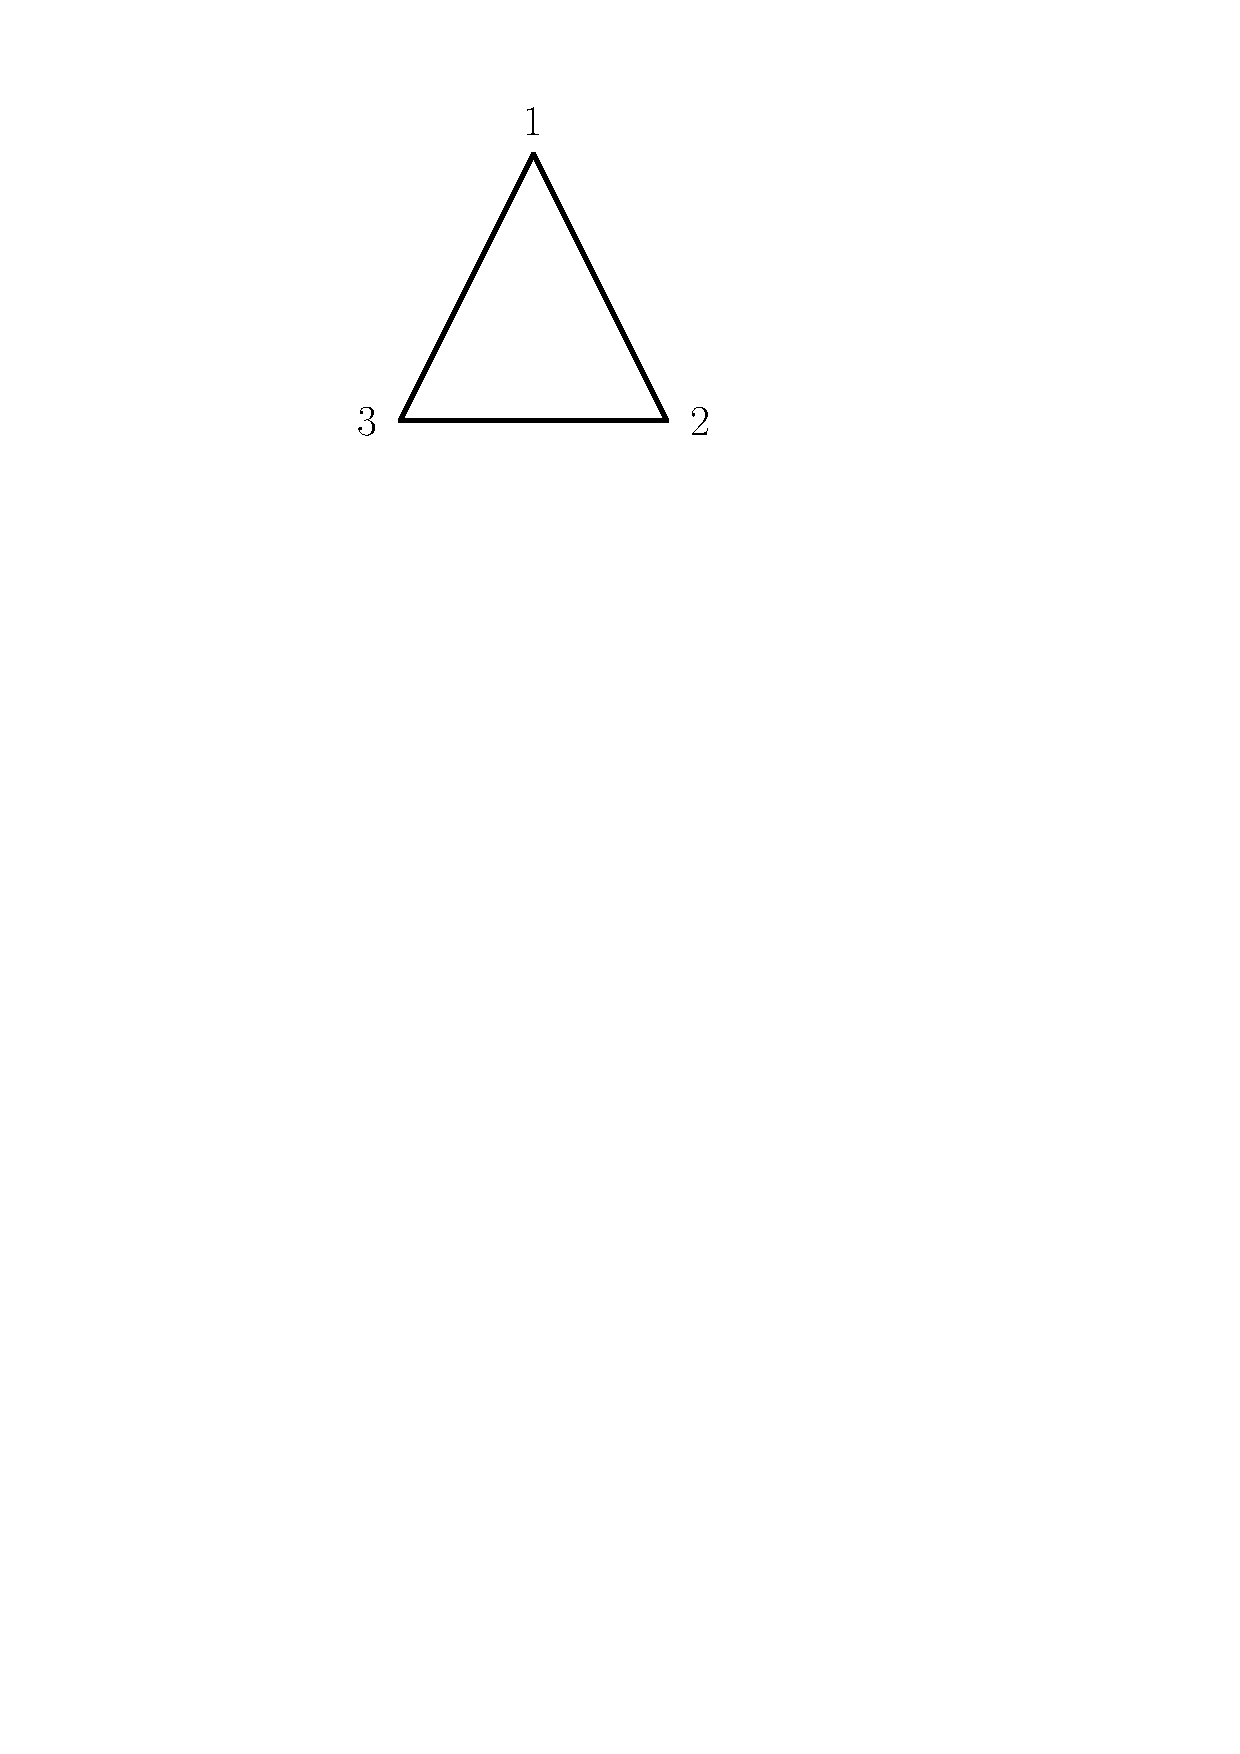
\includegraphics[width=0.25\linewidth]{triangle (1).pdf}
    \end{figure*}\\
    The symmetries are
    \begin{align*}
        e:& \quad \emptyset\\
        \alpha: & \quad 1 \rightarrow 2 \rightarrow 3 \rightarrow 1\\
        \beta: & \quad 1 \rightarrow 3 \rightarrow 2 \rightarrow 1\\
        \gamma: & \quad 1 \leftrightarrow 2\\
        \lambda: & \quad 1 \leftrightarrow 3\\
        \omega: & \quad 2 \leftrightarrow 3
    \end{align*}
    The compositions of these symmetries we compute as:
    \begin{table}[ht]
        \centering
        \begin{tabular}{c|cccccc}
            $\circ$ & $e$ & $\alpha$ & $\beta$ & $\gamma$ & $\lambda$ & $\omega$\\
            \hline
            $e$ & $e$ & $\alpha$ & $\beta$ & $\gamma$ & $\lambda$ & $\omega$\\
            $\alpha$ & $\alpha$ & $\beta$ & $e$ & $\omega$ & $\gamma$ & $\lambda$\\
            $\beta$ & $\beta$ & $e$ & $\alpha$ & $\lambda$ & $\omega$ & $\gamma$\\
            $\gamma$ & $\gamma$ & $\lambda$ & $\omega$ & $e$ & $\alpha$ & $\beta$\\
            $\lambda$ & $\lambda$ & $\omega$ & $\gamma$ & $\beta$ & $e$ & $\alpha$\\
            $\omega$ & $\omega$ & $\gamma$ & $\lambda$ & $\alpha$ & $\beta$ & $e$
        \end{tabular}
    \end{table}
    
    \pagebreak
    \begin{center}
        {\Huge \color{red} Extra} {\Large \color{green} credit} {\color{blue} bonus} {\small \color{yellow} question}
    \end{center}
\end{document}